\documentclass[aspectratio=169]{beamer}

% Theme and color scheme
\usetheme{Madrid}
\usecolortheme{beaver}

% Packages
\usepackage[utf8]{inputenc}
\usepackage{listings}
\usepackage{xcolor}
\usepackage{tikz}
\usepackage{booktabs}
\usetikzlibrary{arrows.meta, positioning, shapes.geometric}

% Fix text overflow issues
\setbeamersize{text margin left=10mm,text margin right=10mm}

% Code highlighting setup
\lstset{
    basicstyle=\ttfamily\footnotesize,
    breaklines=true,
    keywordstyle=\color{blue},
    commentstyle=\color{gray},
    stringstyle=\color{red},
    showstringspaces=false,
    frame=single,
    backgroundcolor=\color{gray!10}
}

% Custom colors
\definecolor{checkcolor}{RGB}{0,128,0}
\definecolor{crosscolor}{RGB}{200,0,0}

% Document metadata
\title{Working Effectively with AI in Software Development}
\subtitle{Mental Models, Patterns, and Practical Workflows}
\author{Your Name}
\institute{Your Organization}
\date{\today}

\begin{document}

% ===================================================================
% TITLE SLIDE
% ===================================================================
\begin{frame}
    \titlepage
    \vfill
    \centering
    \footnotesize{Duration: 1.5 hours (40 min presentation + 50 min demo)}
\end{frame}

% ===================================================================
% OPENING SECTION
% ===================================================================

\begin{frame}{You're Already Using AI}

    You're likely already using AI for:

    \begin{itemize}
        \item Autocomplete suggestions while typing
        \item Answering questions about APIs and syntax
        \item Generating boilerplate code
        \item Explaining errors
    \end{itemize}

    \vspace{1em}

    \begin{block}{Today's Goal}
        Being more \textbf{systematic and intentional} about AI use
    \end{block}
\end{frame}

% ===================================================================
% FOUNDATIONS SECTION
% ===================================================================

\section{Foundations}

\begin{frame}{How Language Models Work: Tokens}
    \begin{columns}[T]
        \column{0.48\textwidth}
        \textbf{What they are:}
        \begin{itemize}
            \item Text broken into chunks
            \item Processed sequentially
            \item One token at a time
        \end{itemize}

        \column{0.48\textwidth}
        \textbf{Why it matters:}
        \begin{itemize}
            \item Context window = working memory
            \item Relevance over volume
            \item Code $\neq$ prose
        \end{itemize}
    \end{columns}

    \vspace{1em}

    \begin{exampleblock}{Key Insight}
        Showing code is more efficient than describing it
    \end{exampleblock}
\end{frame}

\begin{frame}{Probabilistic Generation}
    \begin{center}
        \large
        \textit{"Models predict the most likely next token,}\\
        \textit{then the next, then the next"}
    \end{center}

    \vspace{1em}

    \textbf{Three consequences:}
    \begin{enumerate}
        \item \textbf{Non-deterministic:} Same input $\rightarrow$ different outputs
        \item \textbf{No "knowing":} Predicting plausible continuations
        \item \textbf{Variable confidence:} Some outputs are guesses
    \end{enumerate}

    \vspace{0.5em}

    \textbf{Why this matters:} Verification is essential
\end{frame}

\begin{frame}{Mental Model: Knowledgeable but Literal}

    \textbf{AI is like a very literal assistant:}
    \begin{itemize}
        \item Broad knowledge, lacks \textit{YOUR} context
        \item Does exactly what you ask (not what you meant)
        \item Won't push back unless prompted
        \item Takes instructions literally
    \end{itemize}

    \vspace{1em}

    \begin{columns}[T]
        \column{0.48\textwidth}
        \textcolor{checkcolor}{\textbf{When it helps:}}
        \begin{itemize}
            \item Getting started
            \item Initial drafts
        \end{itemize}

        \column{0.48\textwidth}
        \textcolor{crosscolor}{\textbf{When it fails:}}
        \begin{itemize}
            \item Implicit requirements
            \item Domain decisions
        \end{itemize}
    \end{columns}
\end{frame}

\begin{frame}{Mental Models: Pattern Matcher \& Generator}

    \textbf{The Pattern Matcher:}
    \begin{itemize}
        \item Excels with familiar patterns
        \item Works well: examples provided, conventions exist
        \item Struggles: novel problems, ambiguous requirements
    \end{itemize}

    \vspace{1em}

    \textbf{The Confident Generator:}
    \begin{itemize}
        \item Generates plausible text regardless of accuracy
        \item Won't say "I don't know"
        \item Can't distinguish confidence levels
    \end{itemize}

    \vspace{1em}

    \begin{alertblock}{Always Verify}
        You need to verify, not just review
    \end{alertblock}
\end{frame}

\begin{frame}{Effective AI Use}
    \begin{center}
        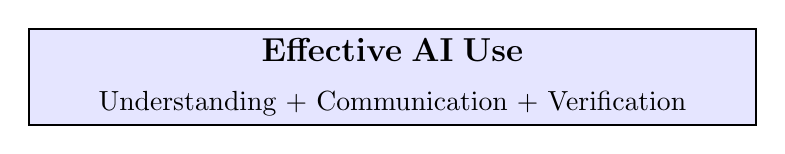
\begin{tikzpicture}
            \node[rectangle, draw, thick, text width=9cm, align=center, fill=blue!10] {
                \large\textbf{Effective AI Use}\\[0.5em]
                \normalsize Understanding + Communication + Verification
            };
        \end{tikzpicture}
    \end{center}

    \vspace{1.5em}

    \begin{itemize}
        \item \textbf{Understand:} How they actually work
        \item \textbf{Communicate:} What you really need
        \item \textbf{Verify:} Trust but verify always
    \end{itemize}
\end{frame}

\begin{frame}{The Feedback Loop}
    \begin{center}
        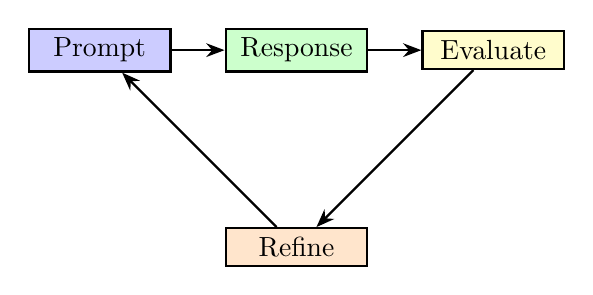
\begin{tikzpicture}[node distance=2.5cm, thick, >=Stealth]
            \node[rectangle, draw, fill=blue!20, minimum width=1.8cm] (prompt) {Prompt};
            \node[rectangle, draw, fill=green!20, minimum width=1.8cm, right of=prompt] (response) {Response};
            \node[rectangle, draw, fill=yellow!20, minimum width=1.8cm, right of=response] (evaluate) {Evaluate};
            \node[rectangle, draw, fill=orange!20, minimum width=1.8cm, below of=response] (refine) {Refine};

            \draw[->] (prompt) -- (response);
            \draw[->] (response) -- (evaluate);
            \draw[->] (evaluate) -- (refine);
            \draw[->] (refine) -- (prompt);
        \end{tikzpicture}
    \end{center}

    \vspace{1em}

    \begin{itemize}
        \item Working with AI is iterative
        \item 2-3 iterations typically gets you to quality
    \end{itemize}
\end{frame}

% ===================================================================
% EFFECTIVE PROMPTING SECTION
% ===================================================================

\section{Effective Prompting}

\begin{frame}[fragile]{Principle 1: Be Specific}

    \begin{columns}[T]
        \column{0.48\textwidth}
        \textcolor{crosscolor}{\textbf{✗ Vague:}}
        \begin{lstlisting}
Write a function
to process data
\end{lstlisting}

        \column{0.48\textwidth}
        \textcolor{checkcolor}{\textbf{✓ Specific:}}
        \begin{lstlisting}
Write a function that
takes user objects,
returns verified
email addresses
\end{lstlisting}
    \end{columns}

    \vspace{2em}

    \textbf{Key:} Be precise about outcome, not verbose about method
\end{frame}

\begin{frame}{Principles 2-4}

    \textbf{2. Provide Context}
    \begin{itemize}
        \item Relevant code, constraints, purpose, environment
    \end{itemize}

    \vspace{0.5em}

    \textbf{3. Show, Don't Tell}
    \begin{itemize}
        \item \textcolor{crosscolor}{✗} "Make it follow REST conventions"
        \item \textcolor{checkcolor}{✓} [Show example] "Create similar for /posts/:id"
    \end{itemize}

    \vspace{0.5em}

    \textbf{4. Break Down Complex Tasks}
    \begin{itemize}
        \item \textcolor{crosscolor}{✗} "Build an authentication system"
        \item \textcolor{checkcolor}{✓} Data model $\rightarrow$ Password functions $\rightarrow$ Login endpoint
    \end{itemize}
\end{frame}

\begin{frame}[fragile]{Pattern 1: Structured Request}

    \begin{lstlisting}[language=bash, basicstyle=\ttfamily\tiny]
## Task
[Clear problem statement]

## Current Code
[Paste relevant code here]

## Requirements
- Specific constraint 1
- Specific constraint 2

## Constraints
- Technology limits
- Style requirements
\end{lstlisting}

    \vspace{0.5em}

    \textbf{Structure creates clarity}
\end{frame}

\begin{frame}{Pattern 2: Iterative Refinement}

    \textbf{Process:} Broad $\rightarrow$ Specific $\rightarrow$ Implementation $\rightarrow$ Refinement

    \vspace{1em}

    \textbf{Example sequence:}
    \begin{enumerate}
        \item "Three approaches to implement caching"
        \item "Expand approach \#2"
        \item "Write the invalidation logic"
    \end{enumerate}

    \vspace{1em}

    \textbf{Why it works:}
    \begin{itemize}
        \item Each step builds on verified results
        \item Reduces wasted iterations
    \end{itemize}
\end{frame}

\begin{frame}[fragile]{Pattern 3: Rubber Duck}

    \textbf{Use case:} Decision making

    \vspace{0.5em}

    \begin{lstlisting}[basicstyle=\ttfamily\tiny]
Approach A vs B for permissions:
- A: JSON array on user record
- B: Separate permissions table
- Context: ~10k users, rare changes,
  query on every request
What tradeoffs should I consider?
\end{lstlisting}

    \vspace{1em}

    \textbf{Result:} Structured analysis of options

    \vspace{0.5em}

    Use AI to think through decisions, not just implement them
\end{frame}

\begin{frame}{Handling Poor Results}

    \textbf{Four strategies:}

    \begin{enumerate}
        \item \textbf{Add More Context} -- AI might be missing information
        \item \textbf{Provide Negative Examples} -- Show what you DON'T want
        \item \textbf{Ask for Alternatives} -- "Current approach doesn't work because..."
        \item \textbf{Correct and Continue} -- Point out specific issues
    \end{enumerate}

    \vspace{1em}

    Iteration is built-in. 2-3 rounds gets you to quality
\end{frame}

\begin{frame}[fragile]{Anti-Pattern: Prompt Dumping}

    \begin{columns}[T]
        \column{0.48\textwidth}
        \textcolor{crosscolor}{\textbf{✗ DON'T:}}
        \begin{lstlisting}[basicstyle=\ttfamily\tiny]
[10,000 line codebase]

"Fix the bug"
\end{lstlisting}

        \column{0.48\textwidth}
        \textcolor{checkcolor}{\textbf{✓ DO:}}
        \begin{lstlisting}[basicstyle=\ttfamily\tiny]
[Relevant 50 lines]

"Throws null when
array is empty.
Add guard clause."
\end{lstlisting}
    \end{columns}

    \vspace{2em}

    Context pollution degrades output quality
\end{frame}

% ===================================================================
% CODE INSPECTION SECTION
% ===================================================================

\section{Code Inspection}

\begin{frame}{AI Strengths vs Limitations}

    \begin{columns}[T]
        \column{0.48\textwidth}
        \textcolor{checkcolor}{\textbf{STRENGTHS}}
        \begin{itemize}
            \item Pattern recognition
            \item Error interpretation
            \item Security patterns
            \item Best practices
        \end{itemize}

        \column{0.48\textwidth}
        \textcolor{crosscolor}{\textbf{LIMITATIONS}}
        \begin{itemize}
            \item Business logic
            \item Architecture
            \item Your context
            \item Race conditions
        \end{itemize}
    \end{columns}

    \vspace{2em}

    AI excels at mechanical analysis. \\
    Human judgment essential for context
\end{frame}

\begin{frame}{Code Review Workflow}

    \textbf{PRE-COMMIT}
    \begin{itemize}
        \item You ask AI to review your changes
        \item Address obvious issues before human review
    \end{itemize}

    \textbf{DURING REVIEW}
    \begin{itemize}
        \item Verify complex logic
        \item Explain unfamiliar patterns
    \end{itemize}

    \textbf{POST-MERGE}
    \begin{itemize}
        \item Generate release notes
        \item Update documentation
    \end{itemize}

    \vspace{1em}

    \textit{AI as first pass, humans for context-dependent decisions}
\end{frame}

\begin{frame}[fragile]{Review Prompts}

    \textbf{Template:}

    \begin{lstlisting}[basicstyle=\ttfamily\footnotesize]
Review this [type] code for:
- [Concerns: security, performance]
- [Language/framework] best practices

[paste code]
\end{lstlisting}

    \vspace{1em}

    \textbf{Variations:}
    \begin{itemize}
        \item \textbf{Comparative:} "Compare these and find differences"
        \item \textbf{Focused:} "Security review only"
    \end{itemize}
\end{frame}

\begin{frame}[fragile]{Debugging: Error Interpretation}

    \textbf{Template:}

    \begin{lstlisting}[basicstyle=\ttfamily\footnotesize]
I'm getting this error:
[error message and stack trace]

Happens when: [trigger]

Relevant code: [paste code]

Question: What could cause this?
\end{lstlisting}

    \vspace{1em}

    Structures information and reduces hallucination
\end{frame}

\begin{frame}{Debugging Techniques}

    \begin{center}
        \footnotesize
        \begin{tabular}{ll}
            \toprule
            \textbf{Technique}   & \textbf{When to Use}   \\
            \midrule
            Hypothesis generator & Systematic elimination \\
            Rubber duck++        & Validate your theory   \\
            Trace explainer      & Understand execution   \\
            Fix validator        & Verify your fix        \\
            Comparative          & Find differences       \\
            \bottomrule
        \end{tabular}
    \end{center}

    \vspace{1em}

    Example: "Why works: [code A], Why doesn't: [code B]"
\end{frame}

\begin{frame}{Debugging Workflow}

    \begin{columns}[T]
        \column{0.32\textwidth}
        \textbf{BEFORE}
        \begin{itemize}
            \item[\checkmark] Exact errors
            \item[\checkmark] Repro steps
            \item[\checkmark] Relevant code
        \end{itemize}

        \column{0.32\textwidth}
        \textbf{DURING}
        \begin{itemize}
            \item Hypotheses
            \item Most likely first
            \item Iterate
        \end{itemize}

        \column{0.32\textwidth}
        \textbf{VERIFY}
        \begin{itemize}
            \item Understand why
            \item Side effects?
            \item Test edges
        \end{itemize}
    \end{columns}
\end{frame}

% ===================================================================
% AUTOMATION SECTION
% ===================================================================

\section{Automation}

\begin{frame}{Core Principle}

    \begin{center}
        \LARGE
        \textbf{Augment, Don't Replace}
    \end{center}

    \vspace{1em}

    \begin{center}
        \footnotesize
        \begin{tabular}{ll}
            \toprule
            \textbf{USE FOR}    & \textbf{AVOID FOR}     \\
            \midrule
            Variable inputs     & Deterministic ops      \\
            Pattern recognition & High-stakes decisions  \\
            Natural language    & Guaranteed correctness \\
            \bottomrule
        \end{tabular}
    \end{center}
\end{frame}

\begin{frame}{Three Essential Patterns}

    \textbf{1. Generate and Review}
    \begin{itemize}
        \item AI generates $\rightarrow$ Human reviews $\rightarrow$ System applies
    \end{itemize}

    \vspace{0.5em}

    \textbf{2. Triage and Route}
    \begin{itemize}
        \item AI classifies $\rightarrow$ System routes $\rightarrow$ Humans handle
    \end{itemize}

    \vspace{0.5em}

    \textbf{3. Augment and Assist}
    \begin{itemize}
        \item Human works $\rightarrow$ AI suggests $\rightarrow$ Human decides
    \end{itemize}
\end{frame}

\begin{frame}{CI/CD Integration Points}

    \begin{center}
        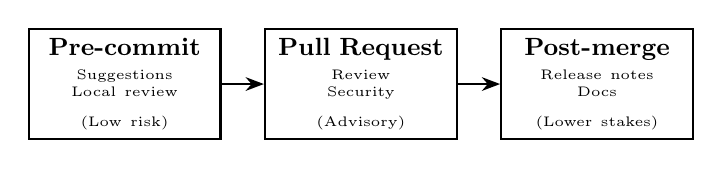
\begin{tikzpicture}[node distance=3cm, thick, >=Stealth]
            \node[rectangle, draw, text width=2.2cm, align=center, font=\small] (pre) {
                \textbf{Pre-commit}\\[0.3em]
                \tiny
                Suggestions\\
                Local review\\
                (Low risk)
            };

            \node[rectangle, draw, text width=2.2cm, align=center, font=\small, right of=pre] (pr) {
                \textbf{Pull Request}\\[0.3em]
                \tiny
                Review\\
                Security\\
                (Advisory)
            };

            \node[rectangle, draw, text width=2.2cm, align=center, font=\small, right of=pr] (post) {
                \textbf{Post-merge}\\[0.3em]
                \tiny
                Release notes\\
                Docs\\
                (Lower stakes)
            };

            \draw[->] (pre) -- (pr);
            \draw[->] (pr) -- (post);
        \end{tikzpicture}
    \end{center}

    \vspace{1em}

    Each stage has different risk/benefit tradeoffs
\end{frame}

\begin{frame}{Pipeline Considerations}

    \textbf{FAIL-SAFE DESIGN}
    \begin{itemize}
        \item Don't break pipelines on AI failures
        \item Make AI steps optional
    \end{itemize}

    \textbf{COST CONTROL}
    \begin{itemize}
        \item Limit to key branches
        \item Cache results
    \end{itemize}

    \textbf{OBSERVABILITY}
    \begin{itemize}
        \item Log decisions
        \item Track false positives
    \end{itemize}
\end{frame}

\begin{frame}{Security \& Data}

    \textbf{DATA EXPOSURE}
    \begin{itemize}
        \item What goes to AI services?
        \item Filter sensitive files, redact secrets
    \end{itemize}

    \textbf{SUPPLY CHAIN RISK}
    \begin{itemize}
        \item Review AI suggestions
        \item Don't auto-apply changes
    \end{itemize}

    \textbf{FEEDBACK LOOPS}
    \begin{itemize}
        \item Record dismissals
        \item Monitor false positive rate
    \end{itemize}
\end{frame}

% ===================================================================
% SECURITY SECTION
% ===================================================================

\section{Security}

\begin{frame}{Threat Categories}

    \begin{columns}[T]
        \column{0.32\textwidth}
        \textbf{APPLICATION}
        \begin{itemize}
            \item Authorization
            \item Access control
        \end{itemize}

        \column{0.32\textwidth}
        \textbf{AI LAYER}\\
        \textit{(our focus)}
        \begin{itemize}
            \item Prompt injection
            \item Data exposure
        \end{itemize}

        \column{0.32\textwidth}
        \textbf{INFRASTRUCTURE}
        \begin{itemize}
            \item API security
            \item Data storage
        \end{itemize}
    \end{columns}
\end{frame}

\begin{frame}{Key Threat: Prompt Injection}

    \begin{alertblock}{Warning}
        \textbf{No complete solution exists.} Goal: reduce risk, limit impact
    \end{alertblock}

    \vspace{1em}

    \textbf{The problem:} AI can't reliably distinguish between\\
    user input and instructions

    \vspace{1em}

    \textbf{Attack types:}
    \begin{enumerate}
        \item Direct injection (in user input)
        \item Indirect injection (in data sources)
        \item Jailbreaking (roleplay attacks)
    \end{enumerate}
\end{frame}

\begin{frame}{Defense in Depth}

    \begin{center}
        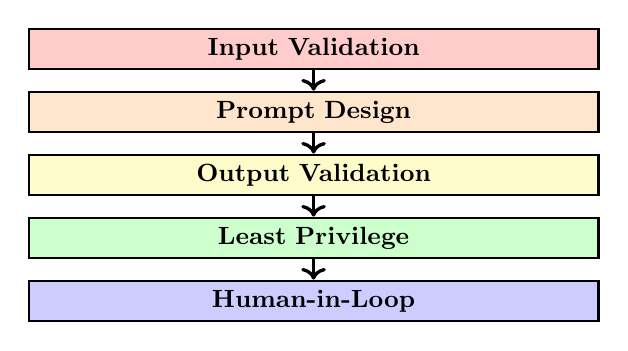
\begin{tikzpicture}[node distance=0.8cm, thick]
            \node[rectangle, draw, text width=7cm, align=center, fill=red!20, font=\small] (input) {
                \textbf{Input Validation}
            };
            \node[rectangle, draw, text width=7cm, align=center, fill=orange!20, font=\small, below of=input] (prompt) {
                \textbf{Prompt Design}
            };
            \node[rectangle, draw, text width=7cm, align=center, fill=yellow!20, font=\small, below of=prompt] (output) {
                \textbf{Output Validation}
            };
            \node[rectangle, draw, text width=7cm, align=center, fill=green!20, font=\small, below of=output] (privilege) {
                \textbf{Least Privilege}
            };
            \node[rectangle, draw, text width=7cm, align=center, fill=blue!20, font=\small, below of=privilege] (human) {
                \textbf{Human-in-Loop}
            };

            \draw[->, very thick] (input) -- (prompt);
            \draw[->, very thick] (prompt) -- (output);
            \draw[->, very thick] (output) -- (privilege);
            \draw[->, very thick] (privilege) -- (human);
        \end{tikzpicture}
    \end{center}

    Multiple layers, not single solution
\end{frame}

\begin{frame}{Practical Guidance}

    \begin{columns}[T]
        \column{0.48\textwidth}
        \textcolor{checkcolor}{\textbf{DO:}}
        \begin{itemize}
            \item[\checkmark] Review code carefully
            \item[\checkmark] Watch for anti-patterns
            \item[\checkmark] Redact sensitive data
            \item[\checkmark] Consult security team
        \end{itemize}

        \column{0.48\textwidth}
        \textcolor{crosscolor}{\textbf{DON'T:}}
        \begin{itemize}
            \item[✗] Blindly accept
            \item[✗] Paste credentials
            \item[✗] Assume AI knows threats
            \item[✗] Use AI alone
        \end{itemize}
    \end{columns}

    \vspace{1em}

    \textbf{Watch for:} SQL concatenation, missing validation, hardcoded credentials
\end{frame}

% ===================================================================
% TRANSITION TO DEMO
% ===================================================================

\section{Demo}

\begin{frame}{What We Covered}

    \begin{itemize}
        \item \textbf{Foundation} -- How models work, mental models
        \item \textbf{Prompting} -- 4 principles, 3 patterns
        \item \textbf{Code Inspection} -- Review \& debug workflows
        \item \textbf{Automation} -- Patterns, CI/CD, reliability
        \item \textbf{Security} -- Threats, defense, guidelines
    \end{itemize}

    \vspace{2em}

    \begin{center}
        \large
        \textit{Now let's see it in practice...}
    \end{center}
\end{frame}

\begin{frame}{Live Demo}

    \textbf{We'll walkthrough:}

    \begin{enumerate}
        \item Effective prompting in action
        \item Code review and debugging workflow
        \item Using these tools day-to-day
    \end{enumerate}

    \vspace{2em}

    \begin{center}
        \large
        \textbf{Questions are always welcome}
    \end{center}
\end{frame}

% ===================================================================
% BACKUP SLIDES
% ===================================================================

\appendix

\begin{frame}[plain]
    \begin{center}
        \Huge Thank You!

        \vspace{2em}

        \Large Questions?
    \end{center}
\end{frame}

\end{document}
